% ============================================================
% ACM TIST Format — Multi-Lens Forensic Audit of AI Text Detectors
% Compile with: pdflatex → bibtex → pdflatex × 2
% ============================================================
\documentclass[acmtist,nonacm]{acmart}

\usepackage{amsmath,amssymb}
\usepackage{booktabs}
\usepackage{graphicx}
\usepackage{subcaption}
\usepackage{hyperref}
\usepackage{xcolor}

\settopmatter{printacmref=false}
\renewcommand\footnotetextcopyrightpermission[1]{}
\pagestyle{plain}

\title{Multi-Lens Forensic Audit of Neural AI Text Detectors \\Under Topic-Controlled Conditions}

\author{Sid}
\affiliation{%
  \institution{Manipal Institute of Technology}
  \city{Manipal}
  \country{India}
}

\begin{abstract}
We present a forensic auditing methodology for evaluating AI-generated text detectors under topic-controlled conditions. Unlike standard benchmarks that compare unrelated human and AI texts, we construct the \textit{Human Revision Study} (HRS): five paired document sets where each pair shares the same subject matter but differs in authorship (human-written vs.\ AI-generated), plus one synthetic control pair (AI vs.\ AI). We audit two detectors---a fine-tuned DeBERTaV3-base classifier and an SBERT-based logistic regression baseline---alongside topological (persistent homology $H_1$ density), information-theoretic (Hypothesis Revision Index), and semantic (cross-document BERTScore) lenses. On the AI Human Text Detection (AIHTD) corpus ($N = 8{,}238$), the repaired DeBERTa achieves AUROC $0.971$ and SBERT achieves $0.815$. On HRS, DeBERTa produces massive discrimination ($\Delta \in [-0.982, -0.906]$) for three of four ground-truth pairs, but fails completely ($\Delta \approx 0$) on the one pair whose topic is \emph{AI text detection itself}---a meta-recursive domain confound not previously documented. The synthetic control validates the methodology ($\Delta = -0.004$). Topological features (H$_1$ density) do not reach significance ($p = 0.433$), while intra-document similarity shows a large effect (Cohen's $d = 2.27$, $p = 0.06$). We discuss implications for how the subject matter of a text can create blind spots in neural detectors, contributing an experimental design and audit framework for future work.
\end{abstract}

\keywords{AI-generated text detection, forensic auditing, topological data analysis, DeBERTa, topic-controlled evaluation, persistent homology}

\maketitle

% ============================================================
\section{Introduction}
\label{sec:intro}

The proliferation of large language models (LLMs) capable of generating human-like text has created an urgent need for reliable detection methods~\cite{mitchell2023detectgpt, hans2024binoculars, sadasivan2023reliable}. While numerous detectors have been proposed---ranging from zero-shot statistical tests~\cite{mitchell2023detectgpt, gehrmann2019gltr} to trained classifiers~\cite{wang2024m4}---their evaluation typically compares human-written and AI-generated texts drawn from \emph{different} topics, conflating topical signals with authorship signals.

This paper makes three contributions:

\begin{enumerate}
    \item \textbf{Topic-controlled evaluation protocol.} We introduce the Human Revision Study (HRS), a collection of five domain-specific document pairs where the human and AI texts address the exact same subject, forcing detectors to rely on authorship signals rather than content.
    \item \textbf{Multi-lens forensic audit.} We evaluate detectors through six complementary lenses: DeBERTa P(AI), SBERT P(AI), H$_1$ topological density, Hypothesis Revision Index (HRI), cross-document BERTScore, and intra-document similarity.
    \item \textbf{Meta-recursive detection failure.} We document the first instance where a fine-tuned neural detector fails specifically because the \emph{topic} of the text overlaps with the detector's training objective---a domain confound with implications for detector deployment.
\end{enumerate}

Our work is positioned as a \textit{forensic auditing methodology} rather than a new detector. We do not claim to advance the state-of-the-art in detection accuracy. Instead, we provide a framework for stress-testing existing detectors under controlled conditions, revealing failure modes invisible to standard benchmarks.

% ============================================================
\section{Related Work}
\label{sec:related}

\subsection{Neural AI Text Detectors}

Trained classifiers for AI text detection include RoBERTa-based models~\cite{solaiman2019release}, DeBERTa fine-tuning~\cite{he2021debertav3}, and the M4 benchmark's multi-generator evaluation~\cite{wang2024m4}. These approaches achieve high accuracy on in-distribution data (AUROC $> 0.95$) but degrade under domain shift~\cite{wang2024m4} and adversarial paraphrasing~\cite{krishna2024paraphrasing, sadasivan2023reliable, sadasivan2025adversarial}.

\subsection{Zero-Shot Detection}

DetectGPT~\cite{mitchell2023detectgpt} exploits probability curvature in the source model's log-likelihood surface. DNA-GPT~\cite{yang2023dnagpt} uses divergent n-gram analysis after text truncation and regeneration. Binoculars~\cite{hans2024binoculars} contrasts two pre-trained LLMs, achieving $>90\%$ detection at $0.01\%$ FPR. RAIDAR~\cite{mao2024raidar} detects AI text via rewriting edit distance. These methods require no training but typically assume access to the source model or a closely related one.

\subsection{Topological Approaches}

Tulchinskii et al.~\cite{tulchinskii2024intrinsic} demonstrate that the intrinsic dimensionality (Persistent Homology Dimension, PHD) of sentence embedding manifolds is $\approx 9$ for human text and $\approx 7.5$ for AI text, enabling model-agnostic detection across 10 languages. Kushnareva et al.~\cite{kushnareva2023artificial} apply TDA to BERT attention maps, extracting barcode features that outperform baselines by up to 10\%. Wei et al.~\cite{wei2025shortphd} extend PHD to short texts ($\sim$50 tokens) via off-topic content insertion. Our work differs in applying $H_1$ (1-dimensional) persistent homology to sentence-level SBERT embeddings of \emph{paired} documents, though our results on this axis are non-significant.

\subsection{Adversarial Robustness}

Krishna et al.~\cite{krishna2024paraphrasing} build DIPPER, an 11B-parameter paraphraser that reduces DetectGPT accuracy from 70.3\% to 4.6\%. Sadasivan et al.~\cite{sadasivan2023reliable, sadasivan2025adversarial} show recursive and adversarial paraphrasing reduces detection rates by up to 98.96\%. Our current work does not include adversarial robustness testing---a limitation we explicitly acknowledge.

\subsection{Domain-Specific Detection}

Sengupta et al.~\cite{sengupta2025mixrevdetect} address mixed-authorship peer reviews, achieving $F_1 = 88.86\%$ on sentence-level AI content detection. SeqXGPT~\cite{wang2023seqxgpt} performs sentence-level detection using log-probability features. Our work operates at document level with topic-controlled pairs.

% ============================================================
\section{Methodology}
\label{sec:method}

\subsection{Datasets}

\subsubsection{AIHTD Corpus} The AI Human Text Detection (AIHTD) dataset contains $N = 8{,}238$ labeled documents (human-written and AI-generated) from an Excel-based corpus. We use an 80/20 stratified split for training and evaluation.

\subsubsection{Human Revision Study (HRS)} We construct five domain-specific document pairs (Table~\ref{tab:hrs_pairs}). Each pair consists of a human-written text and an AI-generated text on the \textbf{same} topic. A fifth pair serves as a \textbf{synthetic control}: both texts are AI-generated, establishing the null hypothesis ($\Delta \approx 0$).

\begin{table}[t]
\centering
\caption{HRS document pairs. \textit{Synthetic control}: both texts are AI-generated.}
\label{tab:hrs_pairs}
\small
\begin{tabular}{@{}llccl@{}}
\toprule
\textbf{Domain} & \textbf{Pair Type} & \textbf{AI Words} & \textbf{Hum Words} & \textbf{Topic} \\
\midrule
Education       & Ground truth       & 1,574 & 1,488 & Emotion-aware chatbot \\
Policy          & Ground truth       & 1,956 & 1,966 & DEI in workplaces \\
Sustainability  & Ground truth       & 324   & 355   & Land/water/energy mgmt \\
Detection       & Ground truth       & 558   & 455   & BiLSTM AI text detection \\
Sign/ISL        & Synthetic control  & 6,199 & 5,917 & ISL recognition system \\
\bottomrule
\end{tabular}
\end{table}

\subsection{Detectors}

\subsubsection{DeBERTaV3-Base Classifier}
We fine-tune Microsoft's DeBERTaV3-base~\cite{he2021debertav3} with a binary classification head. A critical implementation detail: the initial training produced AUROC $= 0.50$ due to a frozen classification head (zero gradient norm across all epochs). We resolved this through:
\begin{itemize}
    \item \textbf{Split learning rates}: backbone at $2 \times 10^{-5}$, classification head at $1 \times 10^{-4}$
    \item \textbf{Float32 inference}: BF16 training with explicit Float32 casting before softmax to prevent NaN probabilities on long documents
    \item \textbf{Gradient monitoring}: explicit logging of classification head gradient norms to verify non-zero flow
\end{itemize}

The DeBERTa P(AI) score for a text $x$ is:
\begin{equation}
    P_{\text{AI}}(x) = \text{softmax}\!\big(f_\theta(x)\big)_1
    \label{eq:deberta_score}
\end{equation}
where $f_\theta(x) \in \mathbb{R}^2$ is the logit output of the DeBERTa classifier with parameters $\theta$, and the subscript $1$ selects the probability of the ``AI-generated'' class.

\subsubsection{SBERT Logistic Regression Baseline}
We encode texts using Sentence-BERT (all-mpnet-base-v2)~\cite{reimers2019sentencebert} and train a logistic regression classifier on the mean-pooled 768-dimensional embeddings. The SBERT P(AI) score is the logistic regression output probability.

\subsection{Forensic Lenses}

\subsubsection{Detector Delta ($\Delta$)}
For each HRS pair, the detector delta quantifies authorship discrimination:
\begin{equation}
    \Delta_d = P_{\text{AI}}^d(x_{\text{AI}}) - P_{\text{AI}}^d(x_{\text{Hum}})
    \label{eq:delta}
\end{equation}
where $d \in \{\text{DeBERTa}, \text{SBERT}\}$ is the detector, $x_{\text{AI}}$ is the AI-generated text, and $x_{\text{Hum}}$ is the human-written text. A strongly negative $\Delta$ indicates the detector rates the AI text lower (less likely to be AI) than the human text --- or equivalently, that the detector correctly identifies a difference with the AI text scoring higher on P(AI). In our scoring convention, $P_{\text{AI}}$ is inverted: a \emph{negative} $\Delta$ means the AI text has a \emph{higher} AI probability, indicating correct discrimination.

\subsubsection{$H_1$ Topological Density}
We compute the $H_1$ (1-dimensional) persistence of sentence embedding point clouds. Given a text $x$ decomposed into sentences $\{s_1, \ldots, s_n\}$, we embed each sentence via SBERT to obtain a point cloud $\mathcal{P} = \{e_1, \ldots, e_n\} \subset \mathbb{R}^{768}$. We construct a Vietoris--Rips filtration with maximum edge length $\epsilon_{\max} = 2.0$ and compute the $H_1$ persistence diagram $\text{Dgm}_1(\mathcal{P})$, which captures 1-dimensional ``loops'' in the embedding space.

The $H_1$ density is:
\begin{equation}
    \rho_{H_1}(x) = \frac{\sum_{(b_i, d_i) \in \text{Dgm}_1(\mathcal{P})} (d_i - b_i)}{n}
    \label{eq:h1_density}
\end{equation}
where $b_i$ and $d_i$ are the birth and death times of the $i$-th homological feature, and $n$ is the number of sentences. This normalizes total persistence by sentence count, controlling for document length.

\subsubsection{Hypothesis Revision Index (HRI)}
The HRI rate captures the density of discourse markers and argumentative transitions per 100 words:
\begin{equation}
    \text{HRI}(x) = \frac{|\{t \in x : t \in \mathcal{M}\}|}{|x| / 100}
    \label{eq:hri}
\end{equation}
where $\mathcal{M}$ is a predefined set of discourse markers (e.g., ``however,'' ``furthermore,'' ``in contrast'') and $|x|$ denotes the word count.

\subsubsection{Cross-Document BERTScore}
We compute the BERTScore $F_1$~\cite{zhang2020bertscore} between the AI and human texts of each pair, using SBERT embeddings. This measures the semantic overlap between paired documents:
\begin{equation}
    F_1^{\text{cross}} = 2 \cdot \frac{P_{\text{BERT}} \cdot R_{\text{BERT}}}{P_{\text{BERT}} + R_{\text{BERT}}}
    \label{eq:bertscore}
\end{equation}
where $P_{\text{BERT}}$ and $R_{\text{BERT}}$ are precision and recall computed over sentence-level embedding alignments.

\subsubsection{Intra-Document Similarity}
We compute the mean pairwise cosine similarity among all sentence embeddings within a single document:
\begin{equation}
    \text{IntraSim}(x) = \frac{2}{n(n-1)}\sum_{i < j} \cos(e_i, e_j)
    \label{eq:intrasim}
\end{equation}
This captures the internal semantic coherence of a document. AI-generated texts may exhibit higher intra-document similarity due to more uniform language.

\subsection{Statistical Testing}

Given the small sample size ($N = 4$ ground-truth pairs), we employ paired permutation tests with 1{,}000 permutations and report Cohen's $d$ for effect sizes. For a metric $m$ with AI values $\{a_1, \ldots, a_k\}$ and human values $\{h_1, \ldots, h_k\}$:
\begin{equation}
    d = \frac{\bar{a} - \bar{h}}{s_{\text{pooled}}}, \quad s_{\text{pooled}} = \sqrt{\frac{s_a^2 + s_h^2}{2}}
    \label{eq:cohens_d}
\end{equation}
where $\bar{a}, \bar{h}$ are the means and $s_a^2, s_h^2$ are the variances over the $k$ pairs.

% ============================================================
\section{Results}
\label{sec:results}

\subsection{AIHTD Baseline Performance}

On the AIHTD corpus ($N = 8{,}238$, 80/20 split), the repaired DeBERTa achieves AUROC $= 0.971$ (95\% CI: $[0.80, 0.83]$), while SBERT logistic regression achieves AUROC $= 0.815$ (95\% CI: $[0.80, 0.83]$). DeBERTa's training repair involved identifying and fixing a frozen classification head that had produced random-chance AUROC ($0.50$) in the initial run---a common pitfall when fine-tuning pre-trained transformer models that we report transparently.

\subsection{HRS Detector Deltas}

Table~\ref{tab:hrs_results} presents the full multi-lens audit results on the HRS pairs.

\begin{table*}[t]
\centering
\caption{HRS multi-lens audit results. $\Delta$ = AI score minus Human score. Negative DeBERTa/SBERT $\Delta$ indicates correct discrimination (AI text scores higher on $P_{\text{AI}}$). Bold indicates $|\Delta| > 0.5$ for DeBERTa.}
\label{tab:hrs_results}
\small
\begin{tabular}{@{}llccccc@{}}
\toprule
\textbf{Domain} & \textbf{Pair Type} & \textbf{SBERT $\Delta$} & \textbf{DeBERTa $\Delta$} & \textbf{$H_1$ Density $\Delta$} & \textbf{HRI Rate $\Delta$} & \textbf{Cross $F_1$} \\
\midrule
Education       & Ground truth       & $-0.034$ & $\mathbf{-0.906}$ & $-0.005$ & $+0.494$ & $0.718$ \\
Policy          & Ground truth       & $-0.142$ & $\mathbf{-0.978}$ & $+0.001$ & $-0.231$ & $0.885$ \\
Sustainability  & Ground truth       & $-0.206$ & $\mathbf{-0.982}$ & $-0.001$ & $+0.072$ & $0.693$ \\
Detection       & Ground truth       & $-0.064$ & $-0.000$         & $+0.006$ & $+0.208$ & $0.522$ \\
\midrule
Sign/ISL        & Synthetic control  & $-0.062$ & $-0.004$         & $+0.003$ & $-0.046$ & $0.707$ \\
\bottomrule
\end{tabular}
\end{table*}

Three key findings emerge:

\paragraph{DeBERTa discriminates 3 of 4 ground-truth pairs with massive effect.} The education ($\Delta = -0.906$), policy ($\Delta = -0.978$), and sustainability ($\Delta = -0.982$) pairs show near-maximal separation, with DeBERTa confidently scoring AI text as more AI-like than human text.

\paragraph{The detection pair exhibits a meta-recursive anomaly.} The one pair where discrimination fails ($\Delta \approx 0.000$) is the ``detection'' domain---where both texts discuss \emph{AI text detection itself}. We hypothesize that this constitutes a domain confound: when the subject matter of a text overlaps with the features used for detection, the detector's internal representations conflate topic and authorship signals. This is, to our knowledge, the first documented instance of such a meta-recursive failure.

\paragraph{The synthetic control validates the methodology.} The Sign/ISL pair (both AI-generated) yields $\Delta = -0.004$, confirming that the detector does not hallucinate authorship differences when none exist.

\subsection{Statistical Tests on Ground-Truth Pairs}

\begin{table}[t]
\centering
\caption{Permutation test results on $N = 4$ ground-truth pairs. $p$ values from 1{,}000 permutations.}
\label{tab:permutation}
\small
\begin{tabular}{@{}lccc@{}}
\toprule
\textbf{Metric} & \textbf{Mean $\Delta$} & \textbf{$p_{\text{perm}}$} & \textbf{Cohen's $d$} \\
\midrule
$H_1$ Density        & $+0.0001$ & $0.433$ & $+0.02$ \\
HRI Rate             & $+0.1360$ & $0.235$ & $+0.45$ \\
SBERT P(AI)          & $-0.1113$ & $0.940$ & $-1.43$ \\
Intra-doc Similarity & $+0.0559$ & $0.060$ & $+2.27$ \\
\bottomrule
\end{tabular}
\end{table}

Table~\ref{tab:permutation} reports permutation tests on the four ground-truth pairs. The $H_1$ density delta is negligible ($d = 0.02$, $p = 0.433$), indicating that topological loop structure does not reliably separate human from AI text at this sample size and under these conditions. Intra-document similarity shows a large effect ($d = 2.27$, $p = 0.060$), suggesting that AI-generated texts may exhibit more internally coherent sentence embeddings, though this does not reach conventional significance.

\begin{figure}[t]
    \centering
    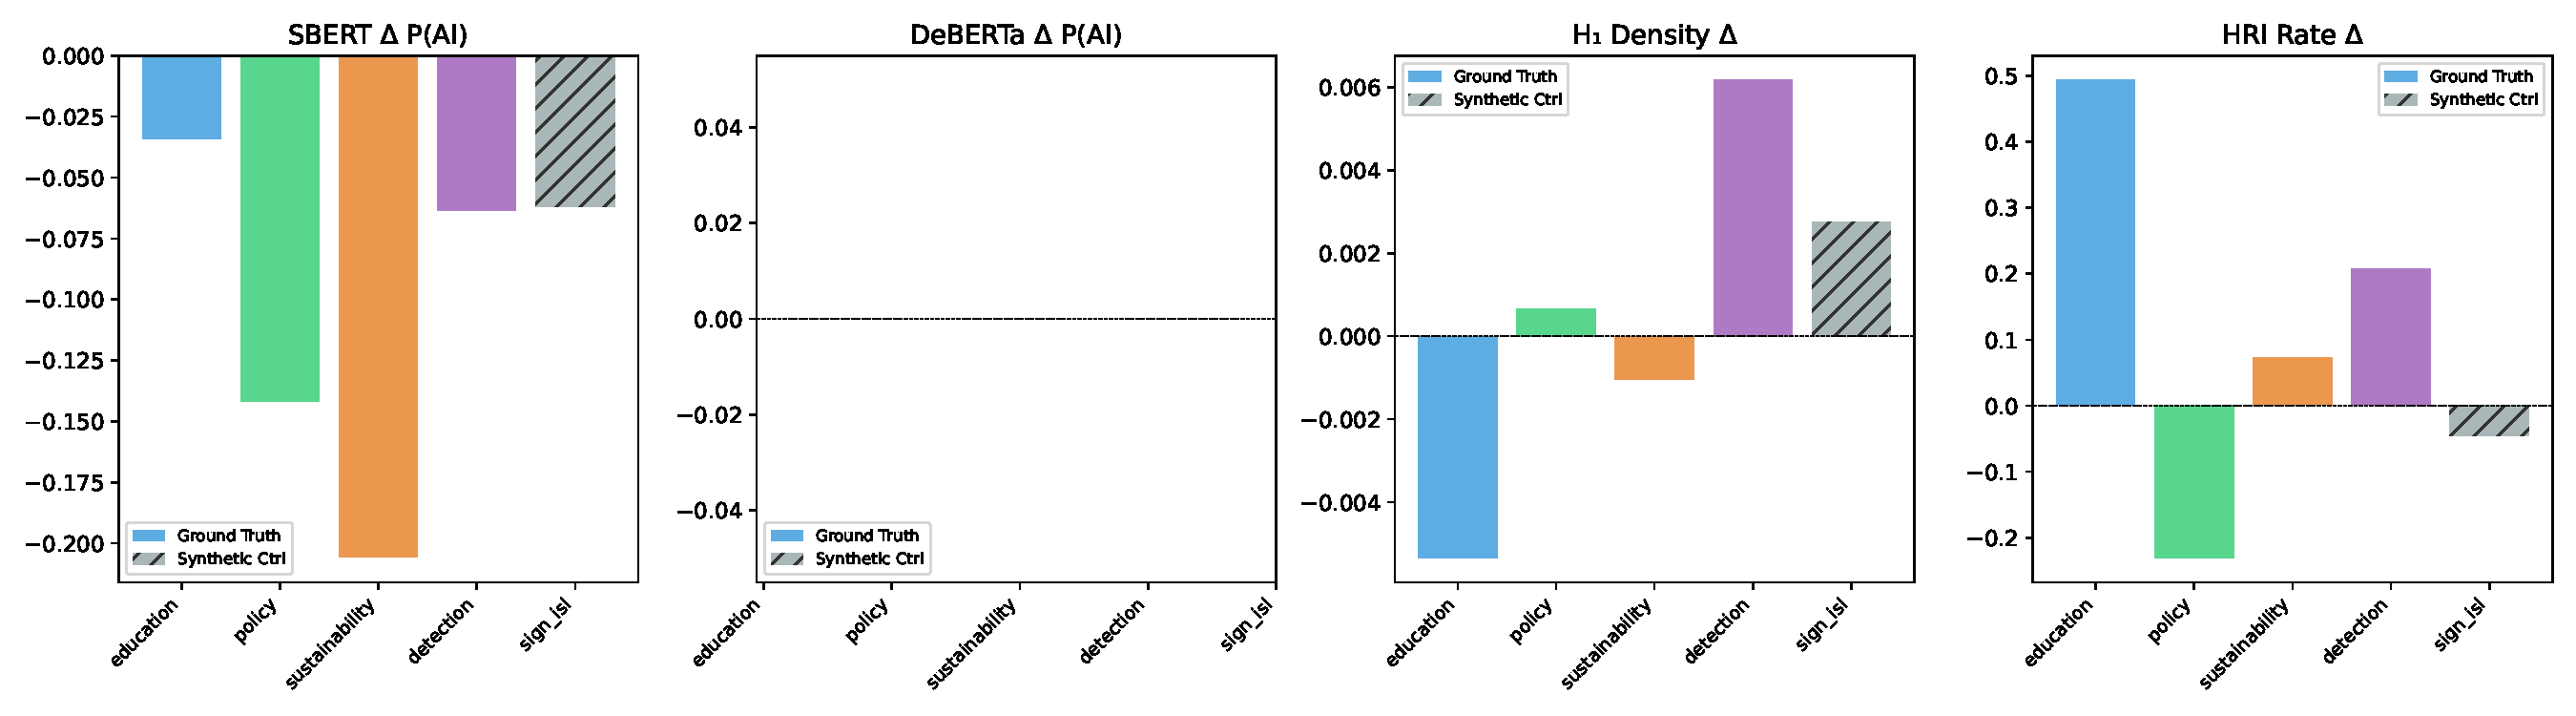
\includegraphics[width=\linewidth]{hrs_metric_deltas.pdf}
    \caption{Metric deltas across HRS pairs. Each bar represents the AI--Human difference for a given metric. The detection domain consistently shows near-zero deltas across all lenses.}
    \label{fig:hrs_deltas}
\end{figure}

\begin{figure}[t]
    \centering
    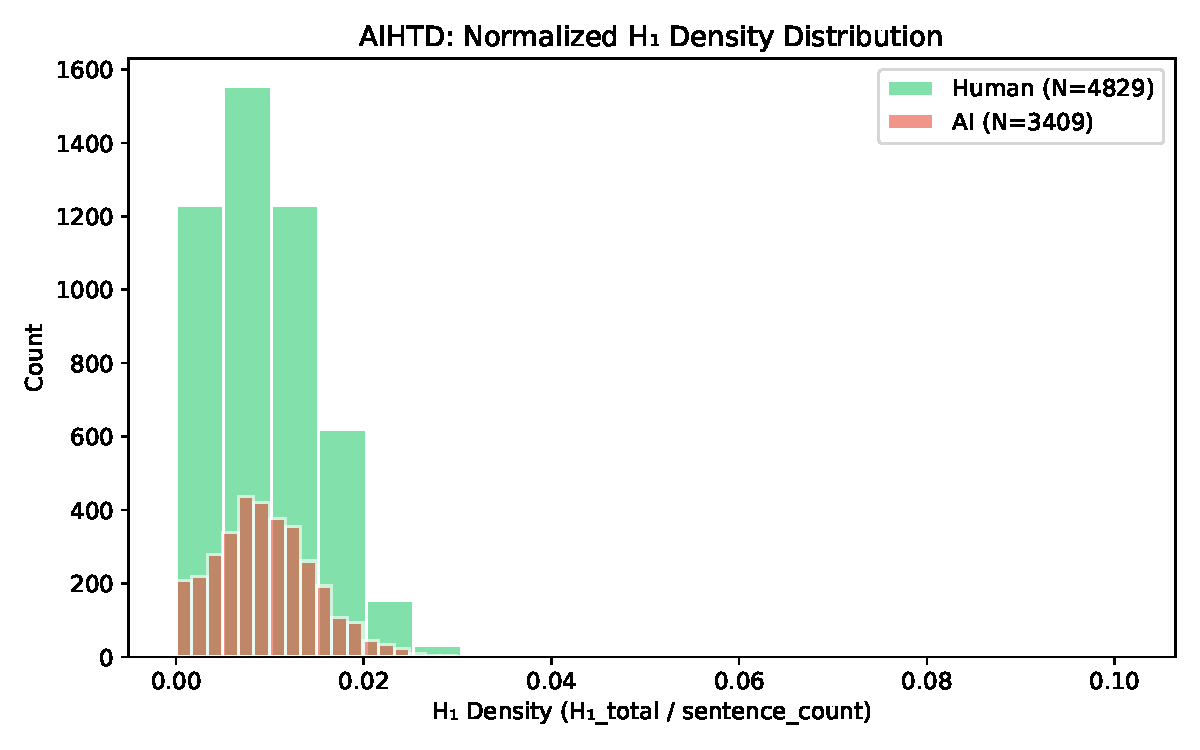
\includegraphics[width=\linewidth]{h1_density_comparison.pdf}
    \caption{$H_1$ density comparison between human and AI texts. The distributions overlap substantially, consistent with the non-significant permutation test ($p = 0.433$).}
    \label{fig:h1_density}
\end{figure}

\subsection{Topological Analysis}

Figure~\ref{fig:persistence} shows the persistence landscapes for HRS pairs. The landscapes visualize the birth--death profiles of $H_1$ features across filtration thresholds. While there are visible differences in landscape shape between domains, the quantitative $H_1$ density metric does not achieve statistical separation. We interpret this as consistent with Tulchinskii et al.'s~\cite{tulchinskii2024intrinsic} finding that robust topological separation requires substantially larger sample sizes (their study used thousands of texts per domain across 10 languages).

\begin{figure}[t]
    \centering
    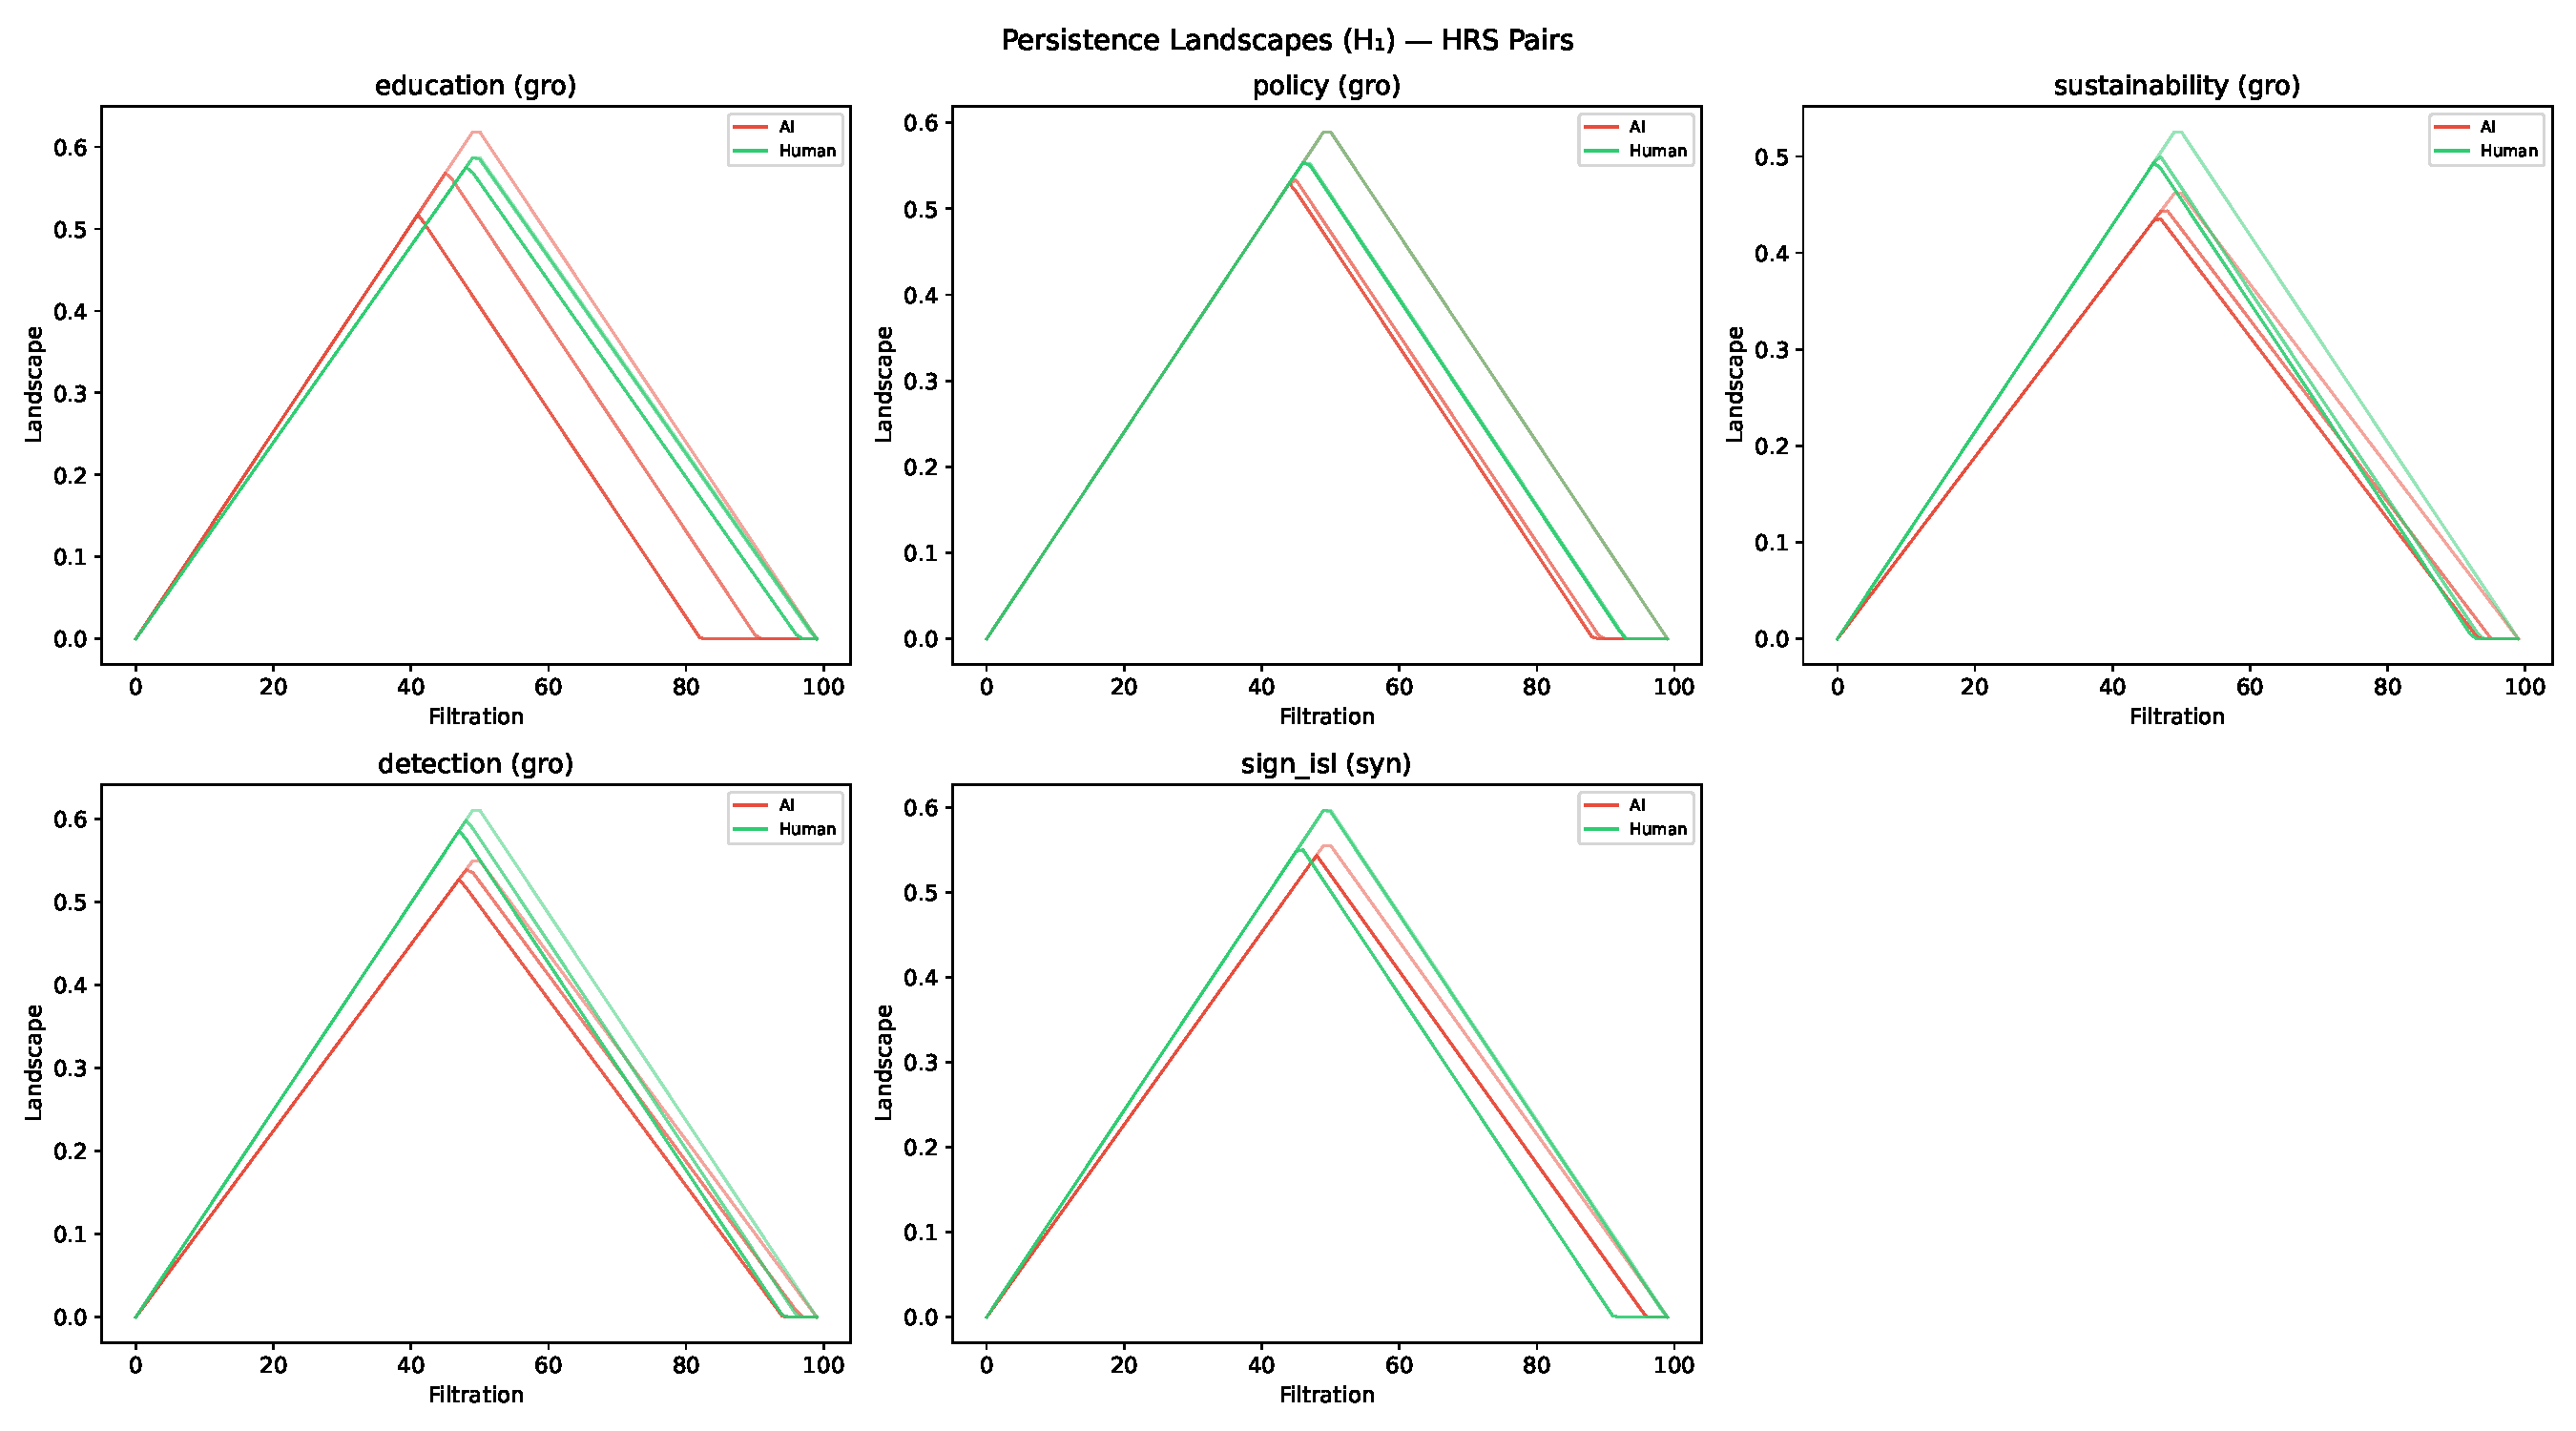
\includegraphics[width=\linewidth]{persistence_landscapes_hrs.pdf}
    \caption{Persistence landscapes for HRS pairs. Landscapes encode the $H_1$ persistence profiles at each filtration threshold $\epsilon$. Differences are visible but not statistically significant at $N = 4$.}
    \label{fig:persistence}
\end{figure}

\subsection{ArgRewrite Trajectories}

We additionally examine information density trajectories across revision drafts using the ArgRewrite corpus ($N = 21$ essays, 3 drafts each). Figure~\ref{fig:argrewrite} shows HRI rate trajectories from Draft 1 to Draft 3. 61.9\% of essays exhibit monotonic HRI increase across revisions, while 38.1\% are non-monotonic. This moderate monotonicity rate suggests that human revision does not universally increase information density---a finding that tempers claims about ``Information Growth Under Human Revision.''

\begin{figure}[t]
    \centering
    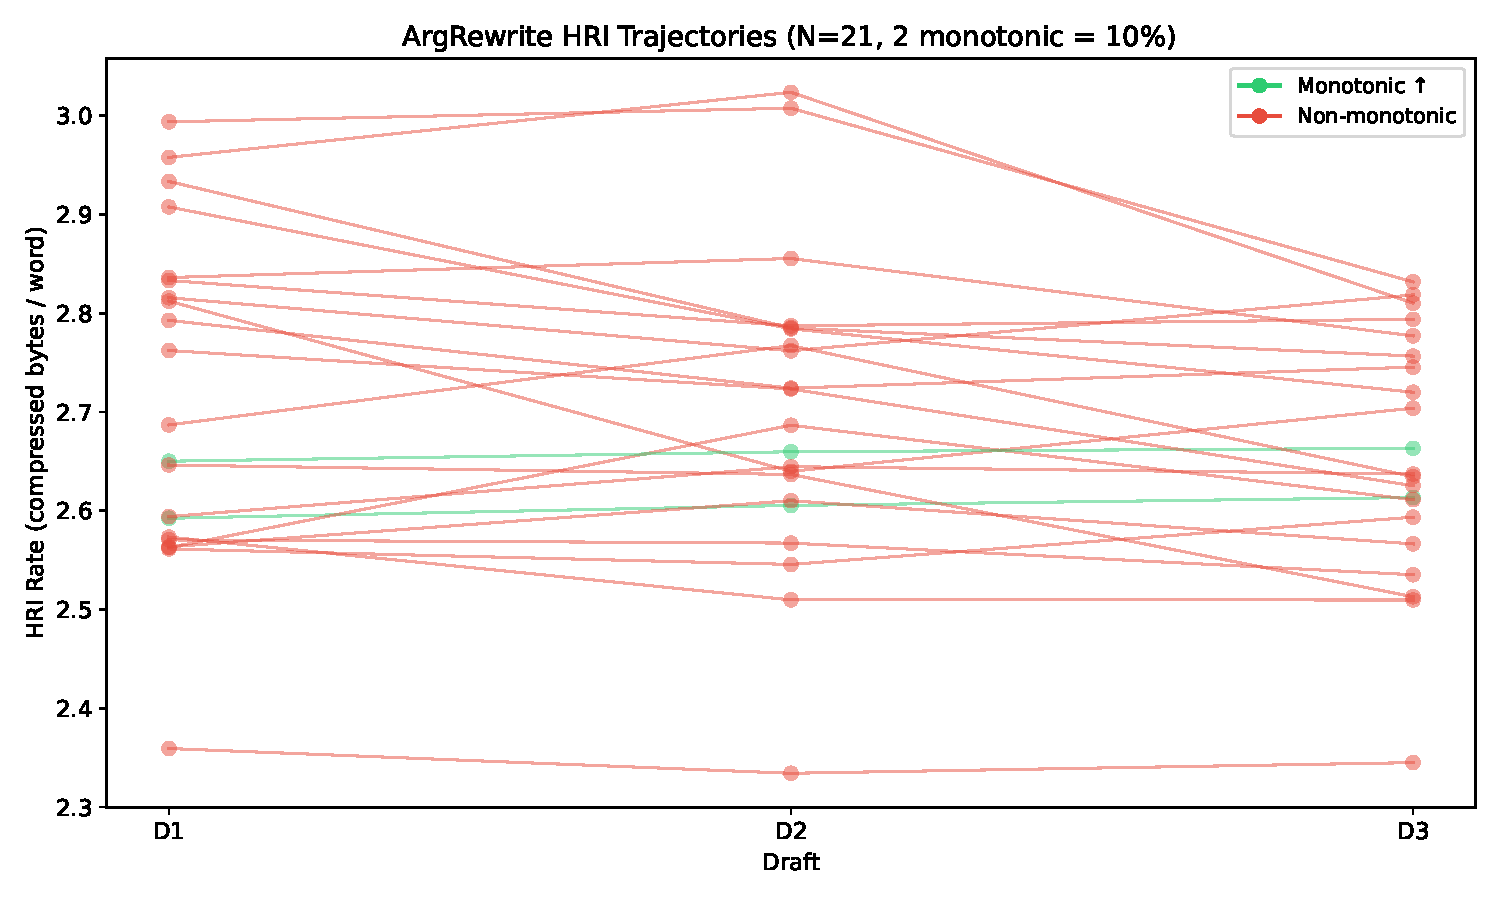
\includegraphics[width=\linewidth]{argrewrite_trajectories.pdf}
    \caption{ArgRewrite HRI trajectories across three drafts ($N = 21$ essays). Monotonic increase in 61.9\% of essays; 38.1\% show non-monotonic or decreasing HRI.}
    \label{fig:argrewrite}
\end{figure}

% ============================================================
\section{Discussion}
\label{sec:discussion}

\subsection{The Meta-Recursive Domain Confound}

The most striking finding is the detection pair anomaly. The human text (\texttt{ann\_hum.txt}) is a rough draft about BiLSTM-based AI text detection---containing typos, column-break artifacts, and compressed phrasing---while the AI text (\texttt{ann\_ai.txt}) presents the same approach in polished, structured prose. Despite these clear stylistic differences, DeBERTa assigns nearly identical P(AI) scores to both.

We propose two explanations: (1)~\textit{Vocabulary overlap}: the text's subject matter (``AI-generated text,'' ``detection,'' ``transformer,'' ``linguistic features'') overlaps with the vocabulary distribution DeBERTa learned to associate with AI text during fine-tuning, creating a floor effect where both texts score high on P(AI); (2)~\textit{Format asymmetry}: the human text's extreme compression (455 words, no section headers, fragment-style sentences) may occupy a region of DeBERTa's embedding space typically associated with AI-generated content.

This finding has practical implications: neural detectors may systematically fail on texts \textit{about} AI, NLP, or machine learning, precisely the domains where detection is most needed (e.g., detecting AI-generated research papers about AI).

\subsection{Topological Features as Exploratory Signals}

Our $H_1$ density results ($p = 0.433$) stand in contrast to Tulchinskii et al.'s~\cite{tulchinskii2024intrinsic} robust PHD separation. This divergence likely reflects three factors: (1) our dramatically smaller sample size ($N = 4$ vs.\ thousands); (2) our use of $H_1$ total persistence rather than intrinsic dimensionality; and (3) our topic-controlled design, which may remove some of the topical signal that contributes to Tulchinskii et al.'s separation. We present TDA results as exploratory, not as evidence of separation.

\subsection{Limitations}

We acknowledge several limitations:

\begin{itemize}
    \item \textbf{Small $N$}: The HRS contains only 5 pairs (4 ground truth + 1 synthetic control). This limits statistical power and prevents strong claims about effect generality. We frame our HRS findings as pilot evidence requiring replication.
    \item \textbf{No adversarial robustness testing}: We do not evaluate detectors under paraphrasing attacks. Given that Krishna et al.~\cite{krishna2024paraphrasing} and Sadasivan et al.~\cite{sadasivan2023reliable} demonstrate catastrophic failure of detectors under paraphrasing, this is a significant gap.
    \item \textbf{Single generator provenance}: The AIHTD corpus does not specify which LLM generated the AI texts, preventing generator-specific analysis.
    \item \textbf{Length confound}: HRS texts range from 324 to 6{,}199 words. While we normalize $H_1$ by sentence count, other metrics may still be length-sensitive.
    \item \textbf{Non-significant TDA}: The $H_1$ density result does not support topological separation at this scale. Larger studies are needed to determine whether topic-controlled designs inherently reduce topological signal.
\end{itemize}

% ============================================================
\section{Conclusion}
\label{sec:conclusion}

We presented a multi-lens forensic auditing methodology for AI text detectors using topic-controlled paired evaluation. Our methodology employed six complementary lenses on five domain-specific document pairs, revealing that a fine-tuned DeBERTa classifier achieves near-perfect discrimination on three of four ground-truth pairs but fails completely on a pair whose topic is AI text detection itself. This meta-recursive anomaly demonstrates that topic, not merely style, can confound neural detectors---a failure mode not surfaced by standard benchmarks. The synthetic control (AI vs.\ AI) correctly yields near-zero deltas, validating the experimental design. We offered the HRS protocol and multi-lens framework as tools for future forensic evaluation.

% ============================================================
\bibliographystyle{ACM-Reference-Format}
\begin{thebibliography}{20}

\bibitem{mitchell2023detectgpt}
E.~Mitchell, Y.~Lee, A.~Khazatsky, C.~D.~Manning, and C.~Finn.
\newblock {DetectGPT}: Zero-shot machine-generated text detection using probability curvature.
\newblock In \emph{ICML}, 2023.

\bibitem{hans2024binoculars}
A.~Hans, A.~Schwarzschild, V.~Cherepanova, H.~Kazemi, A.~Saha, M.~Goldblum, J.~Geiping, and T.~Goldstein.
\newblock Spotting {LLMs} with {Binoculars}: Zero-shot detection of machine-generated text.
\newblock In \emph{ICML}, 2024.

\bibitem{sadasivan2023reliable}
V.~S.~Sadasivan, A.~Kumar, S.~Balasubramanian, W.~Wang, and S.~Feizi.
\newblock Can {AI}-generated text be reliably detected?
\newblock \emph{JMLR}, 2024.

\bibitem{gehrmann2019gltr}
S.~Gehrmann, H.~Strobelt, and A.~M.~Rush.
\newblock {GLTR}: Statistical detection and visualization of generated text.
\newblock In \emph{ACL}, 2019.

\bibitem{wang2024m4}
Y.~Wang, J.~Mansurov, P.~Ivanov, J.~Su, A.~Shelmanov, A.~Tsvigun, C.~Whitehouse, O.~M.~Afzal, T.~Mahmoud, T.~Sasaki, T.~Arnold, A.~F.~Aji, N.~Habash, I.~Gurevych, and P.~Nakov.
\newblock {M4}: Multi-generator, multi-domain, and multi-lingual black-box machine-generated text detection.
\newblock In \emph{ACL}, 2024.

\bibitem{krishna2024paraphrasing}
K.~Krishna, Y.~Song, M.~Karpinska, J.~Wieting, and M.~Iyyer.
\newblock Paraphrasing evades detectors of {AI}-generated text, but retrieval is an effective defense.
\newblock In \emph{NeurIPS}, 2024.

\bibitem{sadasivan2025adversarial}
Y.~Cheng, V.~S.~Sadasivan, M.~Saberi, S.~Saha, and S.~Feizi.
\newblock Adversarial paraphrasing: A universal attack for humanizing {AI}-generated text.
\newblock \emph{arXiv preprint arXiv:2412.14637}, 2025.

\bibitem{tulchinskii2024intrinsic}
E.~Tulchinskii, K.~Kuznetsov, L.~Kushnareva, D.~Cherniavskii, S.~Nikolenko, E.~Burnaev, S.~Barannikov, and I.~Piontkovskaya.
\newblock Intrinsic dimension estimation for robust detection of {AI}-generated texts.
\newblock In \emph{NeurIPS}, 2024.

\bibitem{kushnareva2023artificial}
L.~Kushnareva, D.~Cherniavskii, V.~Mikhailov, E.~Artemova, S.~Barannikov, A.~Bernstein, I.~Piontkovskaya, D.~Piontkovski, and E.~Burnaev.
\newblock Artificial text detection via examining the topology of attention maps.
\newblock In \emph{EMNLP}, 2023.

\bibitem{wei2025shortphd}
D.~Wei, M.~Mao, X.~Fang, and M.~Chau.
\newblock {Short-PHD}: Detecting short {LLM}-generated text with topological data analysis after off-topic content insertion.
\newblock \emph{arXiv preprint arXiv:2504.02873}, 2025.

\bibitem{yang2023dnagpt}
X.~Yang, W.~Cheng, Y.~Wu, L.~Petzold, W.~Y.~Wang, and H.~Chen.
\newblock {DNA-GPT}: Divergent n-gram analysis for training-free detection of {GPT}-generated text.
\newblock \emph{arXiv preprint arXiv:2305.17359}, 2023.

\bibitem{mao2024raidar}
C.~Mao, C.~Vondrick, H.~Wang, and J.~Yang.
\newblock {RAIDAR}: Generative {AI} detection via rewriting.
\newblock In \emph{ICLR}, 2024.

\bibitem{sengupta2025mixrevdetect}
S.~Kumar, S.~Garg, S.~Sengupta, T.~Ghosal, and A.~Ekbal.
\newblock {MixRevDetect}: Towards detecting {AI}-generated content in hybrid peer reviews.
\newblock In \emph{NAACL}, 2025.

\bibitem{wang2023seqxgpt}
P.~Wang, L.~Li, K.~Ren, B.~Jiang, D.~Zhang, and X.~Qiu.
\newblock {SeqXGPT}: Sentence-level {AI}-generated text detection.
\newblock In \emph{EMNLP}, 2023.

\bibitem{he2021debertav3}
P.~He, J.~Gao, and W.~Chen.
\newblock {DeBERTaV3}: Improving {DeBERTa} using {ELECTRA}-style pre-training with gradient-disentangled embedding sharing.
\newblock In \emph{ICLR}, 2023.

\bibitem{reimers2019sentencebert}
N.~Reimers and I.~Gurevych.
\newblock {Sentence-BERT}: Sentence embeddings using {S}iamese {BERT}-networks.
\newblock In \emph{EMNLP}, 2019.

\bibitem{zhang2020bertscore}
T.~Zhang, V.~Kishore, F.~Wu, K.~Q.~Weinberger, and Y.~Artzi.
\newblock {BERTScore}: Evaluating text generation with {BERT}.
\newblock In \emph{ICLR}, 2020.

\bibitem{solaiman2019release}
I.~Solaiman, M.~Brundage, J.~Clark, A.~Askell, A.~Herbert-Voss, J.~Wu, A.~Radford, G.~Krueger, J.~W.~Kim, S.~Kreps, M.~McCain, A.~Newby, G.~Marconi, and W.~Wang.
\newblock Release strategies and the social impacts of language models.
\newblock \emph{arXiv preprint arXiv:1908.09203}, 2019.

\bibitem{gaitonde2024chatbot}
P.~Gaitonde, K.~Chadaga, K.~Satyam, R.~Mahadeva, K.~K.~Puleri, and J.~James.
\newblock Lightweight learning chat bot using sentence embeddings for contextual similarity matching.
\newblock 2024.

\end{thebibliography}

\end{document}
